\documentclass[12pt, twoside]{article}
\usepackage[francais]{babel}
\usepackage[T1]{fontenc}
\usepackage[latin1]{inputenc}
\usepackage[left=1cm, right=1cm, top=1cm, bottom=1cm]{geometry}
\usepackage{float}
\usepackage{graphicx}
\usepackage{array}
\usepackage{multirow}
\usepackage{amsmath,amssymb,mathrsfs}
\usepackage{soul}
\pagestyle{empty}

\begin{document}

\begin{flushright}
$2^{de}5$
\end{flushright}
\begin{center}
\textbf{\large{Devoir Maison 5}}
\end{center}

\textit{Devoir � rendre sur feuille double grand format petits carreaux pour le
\ul{samedi 13 d�cembre 2008}.}
\bigskip
\bigskip


\textbf{Exercice 1:} Faire l'exerice $n^{0}$49 p188 de votre livre.

\medskip

\textit{Remarque:} La figure exacte fera partie du bar�me.

\bigskip


\textbf{Exercice 2:} Recopier et compl�ter:

$(\ldots+5)^{2}=49x^{2}+\ldots+\ldots$

$(3x- \ldots)^{2}=\ldots -24x+\ldots$

$(9x+\ldots)(9x-\ldots)=\ldots-9$

$(4x+\ldots)^{2}=\ldots+8xy+\ldots$

\medskip

\textit{Remarque:} Cet exercice est suffisament simple pour �tre compris par
\ul{tous} les �l�ves de la classe. Il faut comprendre et savoir refaire ce type
de manipulation pour le reste de l'ann�e.

\bigskip

\textbf{Exercice 3:} R�soudre les �quations suivantes:
\begin{enumerate}
  \item $(x-3)^{2}-36=0$
  \item $(2x-1)(x-6)-3(1-2x)-1=2x$
  \item $\dfrac{(7x+2)(x-1)}{3x+5}=0$
\end{enumerate}

\bigskip

\textbf{Exercice 4:} Soit $ABCD$ un carr� de c�t� $5+a$. L'aire du polyg�ne
color� est $36cm^{2}$. Trouver le p�rim�tre du carr� $ABCD$.
\begin{center}
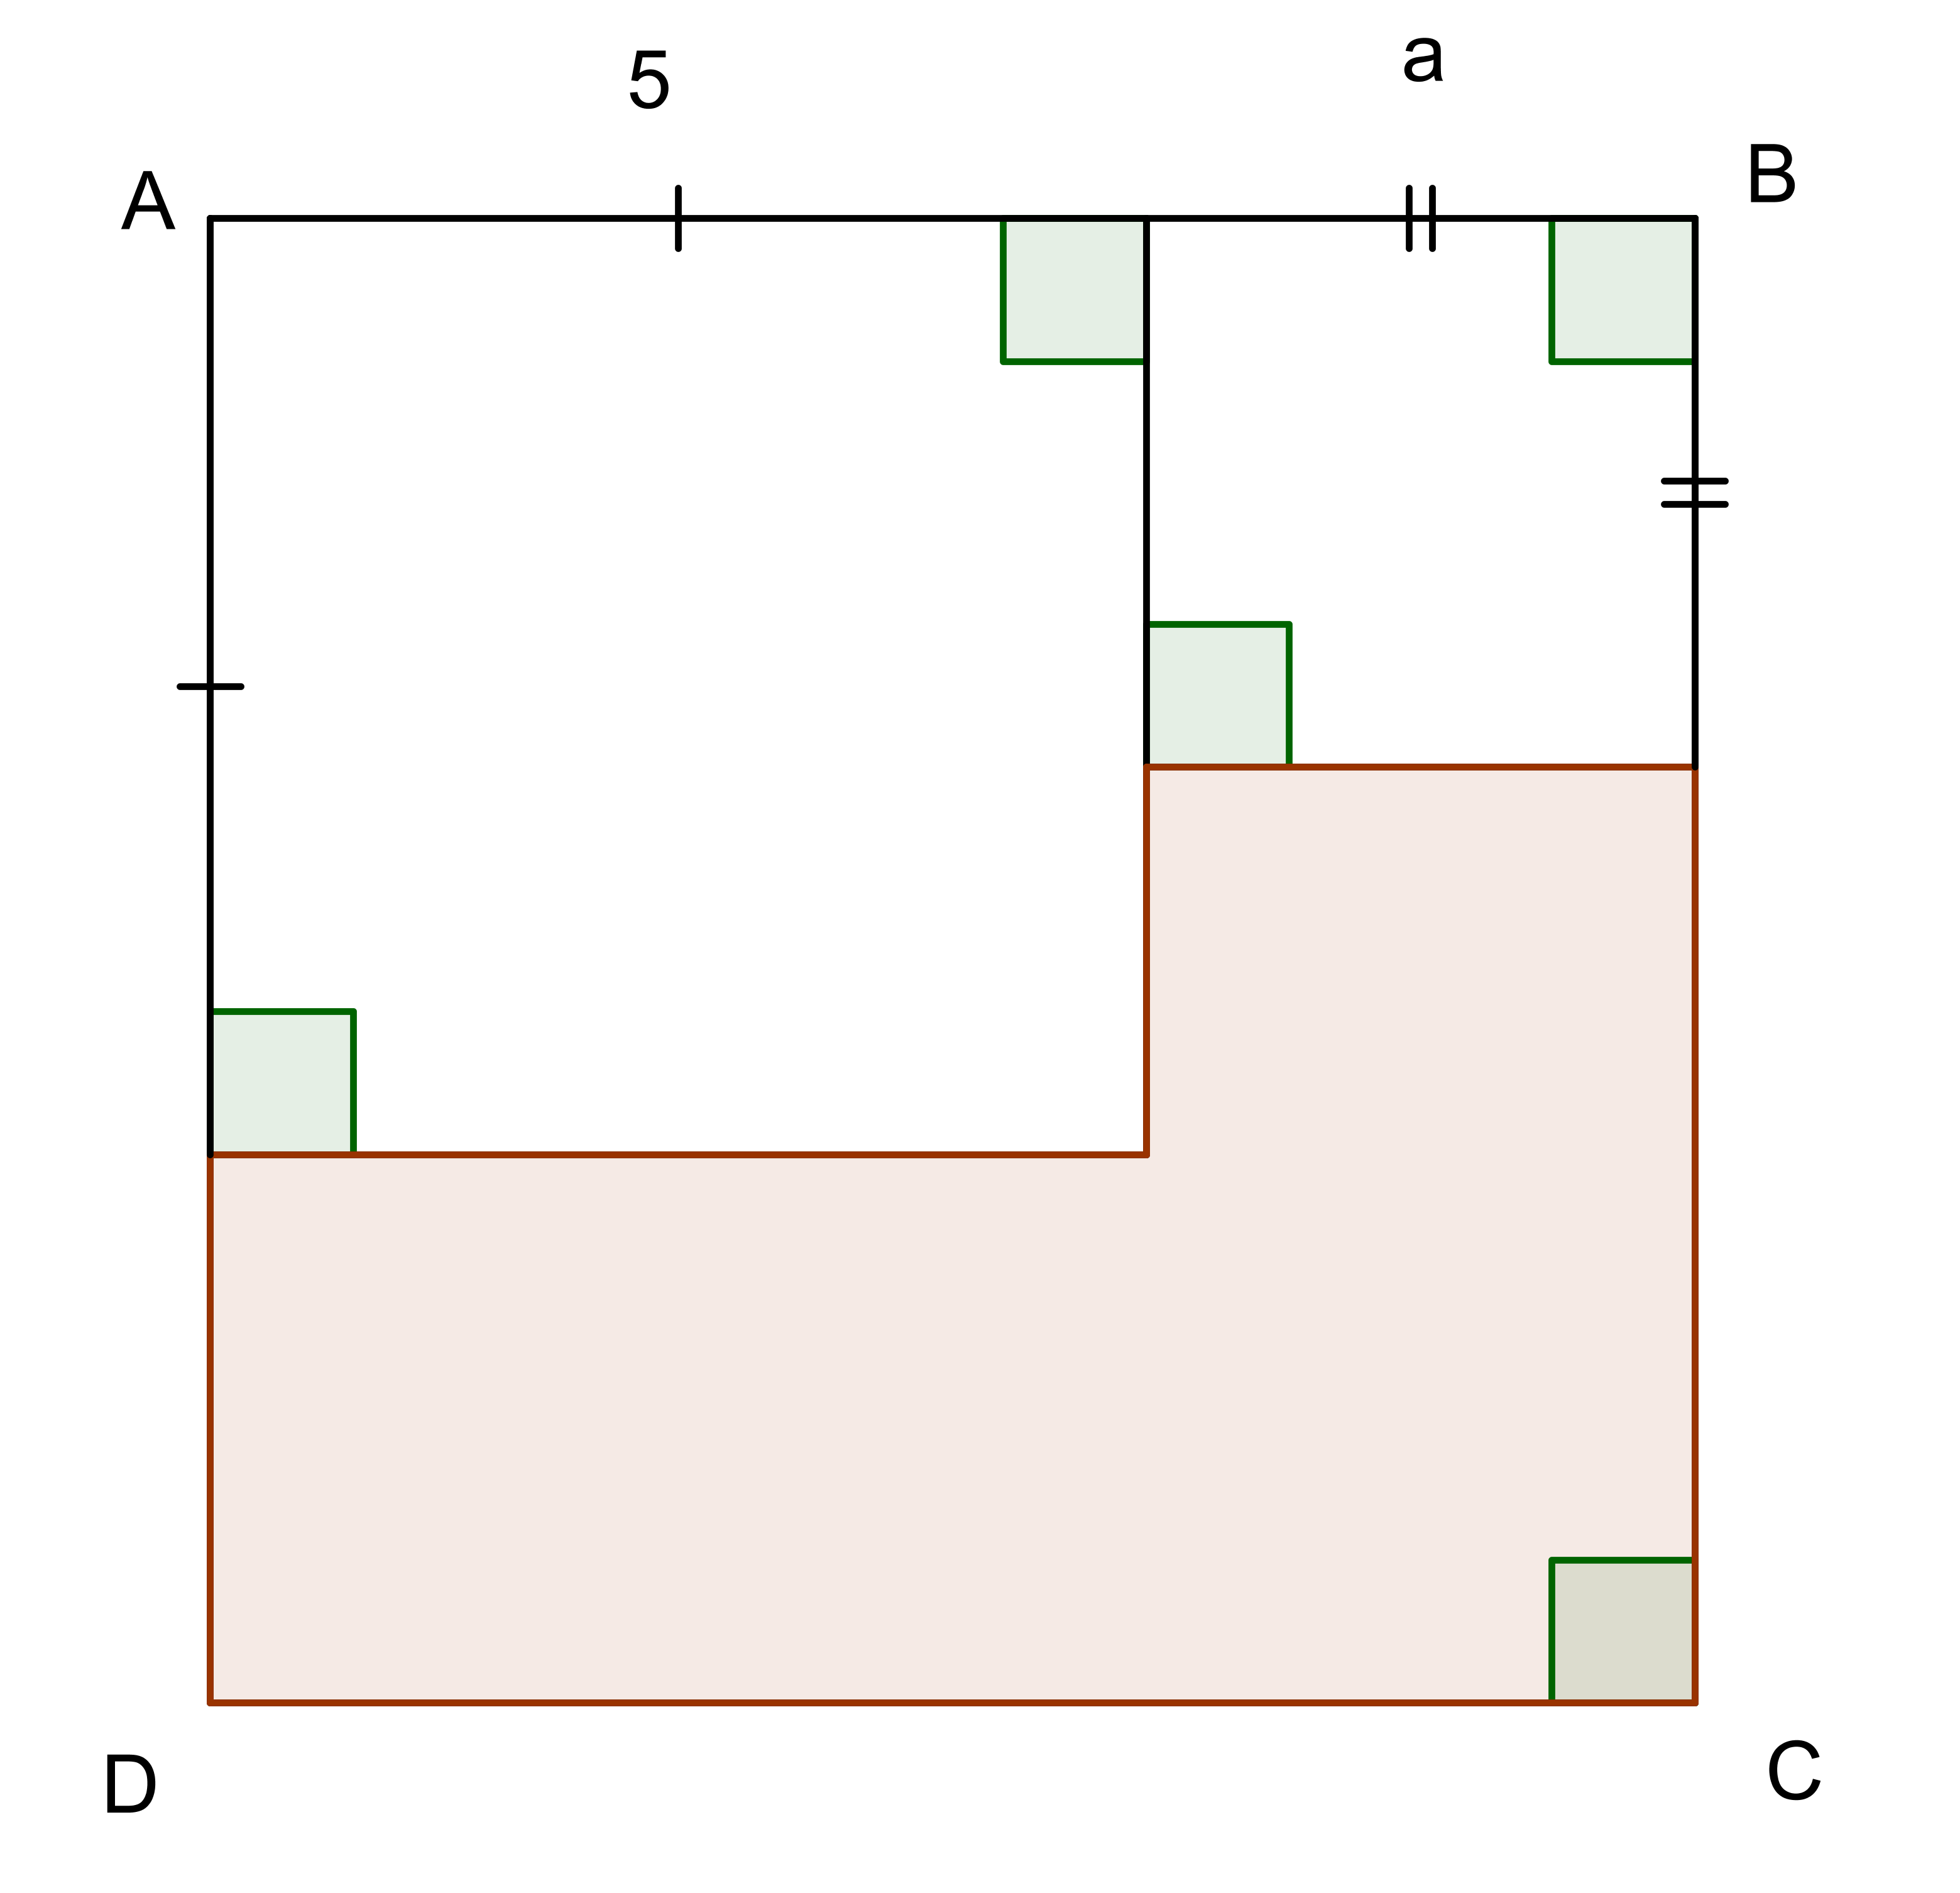
\includegraphics[width=6cm]{image/ex.png}
\end{center}

\bigskip

\textbf{Exercice 5:}
\begin{enumerate}
  \item Soit x un nombre r�el. Factoriser $x^{2}+4x+4$. En d�duire une �criture
  de $x^{2}+4x$ puis de $x^{2}+4x-5$.
  \item R�soudre $(E): \ x^{2}+4x-5=0$.
  \item En rempla�ant x par la (ou les) solution(s) trouv�e(s), v�rifier si vos
  r�sultats sont bien solution de $(E)$ (il s'agit simplement de contr�ler
  le r�sultat trouv� par le calcul).
  \item \ul{BONUS}: Par le m�me raisonnement, r�soudre l'�quation
  $9x^{2}+3x-2=0$.
\end{enumerate}
\end{document}
